% !TEX root = ../Thesis.tex
%
%\documentclass{article}
%\usepackage{graphicx,tikz}
%\usepackage[graphics,tightpage,active]{preview}
%\PreviewEnvironment{tikzpicture}
%\begin{document}
%%%%%%%%%%%%%%%%%%%%%%%%%%%%%%%%%%%%%%%%%%%%%%%%%
	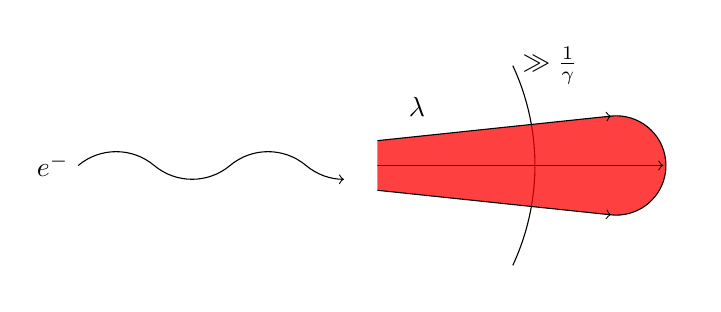
\begin{tikzpicture}
		%\draw [help lines] (0,0) grid (5,5);
		\def\a{130}	% 90+60
		\def\b{50}		% 90-40 
		\def\c{-130}
		\def\d{-50}
		\def\length{0.75}
		\def\start{-0.8}
		% travelling electron
			\node [anchor=east] at (\start,0) {$e^{-}$};
			\draw [->] (\start,0) arc (\a:\b:\length) arc (\c:\d:\length) arc (\a:\b:\length) arc (\c:-90:\length);
		% beam angle
		\clip (3,-1.5) rectangle (7,1.75);
			\draw (5,0) arc (0:-25:3);
			\draw (5,0) arc (0:25:3) node [right] {$\gg\frac{1}{\gamma}$};
		% beam
			\def\alpha{6}
			\def\length{6}
			\def\arclength{0.63062541159405877506901428083929} % arclength = tan(\alpha)*\length
			\fill [color=red,nearly opaque] (0,0) -- (\alpha:\length) arc (90+\alpha:-90-\alpha:\arclength) -- cycle; 
			\draw (\alpha:\length) arc (90+\alpha:-90-\alpha:\arclength);
			\node at (3.5,.75) {$\lambda$};
		% arrows
			\draw [->] (0,0) -- (\alpha:\length);
			\draw [->] (0,0) -- (\length+\arclength,0);
			\draw [->] (0,0) -- (-\alpha:\length);
	\end{tikzpicture}
%%%%%%%%%%%%%%%%%%%%%%%%%%%%%%%%%%%%%%%%%%%%%%%%%
%\end{document}